\documentclass[10pt]{book}
\usepackage{amsmath}
\usepackage{amssymb}
\usepackage[margin=1in]{geometry}
\usepackage{graphicx}
\usepackage{setspace}
\usepackage{textcomp}
\usepackage{verbatim}
\usepackage{mathtools}
\usepackage{enumitem}
\usepackage{complexity}
\usepackage{tikz}
\usepackage{cleveref}

% For drawing stuff
\usetikzlibrary{automata,positioning}

\setlistdepth{9}

\title{Introduction to the Theory of Computation Solutions}
\author{Ryan Dougherty}
\date{}

\newcommand{\alreadyanswered}{answered in the text.}

\newcommand{\angles}[1]{\textlangle{}$#1$\textrangle{}}

\singlespace

\begin{document}
\maketitle

\tableofcontents

\chapter{Solutions}
\section{Chapter 1}

\begin{enumerate}

%		1.1		%
\item[1.1]The following are the state diagrams of two DFAs, $M_1$ and $M_2$. Answer the following questions about each of these machines.
\\
\textbf{Solution:} \alreadyanswered

%		1.2		%
\item[1.2]Give the formal description of the machines $M_1$ and $M_2$ pictured in Exercise 1.1.
\\
\textbf{Solution:} \alreadyanswered

%		1.3		%
\item[1.3]The formal description of a DFA $M$ is $(\{q_1, q_2, q_3, q_4, q_5\}, \{u, d\}, \delta, q_3, \{q_3\})$, where $\delta$ is given by the following table. Give the state diagram of this machine.
\begin{table}[!htb]
\centering
\begin{tabular}{l|ll}
      & $u$   & $d$   \\ \hline
$q_1$ & $q_1$ & $q_2$ \\
$q_2$ & $q_1$ & $q_3$ \\
$q_3$ & $q_2$ & $q_4$ \\
$q_4$ & $q_3$ & $q_5$ \\
$q_5$ & $q_4$ & $q_5$
\end{tabular}
\end{table}

\textbf{Solution:} 
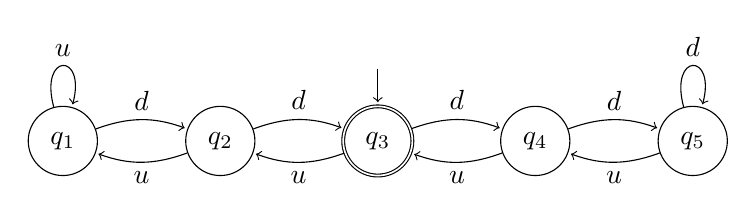
\begin{tikzpicture}[shorten >=1pt,node distance=2cm,initial text={},on grid,auto] 
   \node[state] (q_1)   {$q_1$}; 
   \node[state] (q_2) [right=of q_1] {$q_2$}; 
   \node[state,initial above,accepting](q_3) [right=of q_2] {$q_3$};
   \node[state] (q_4) [right=of q_3] {$q_4$};
   \node[state] (q_5) [right=of q_4] {$q_5$};
    \path[->] 
    (q_1) edge [loop above] node {$u$} (q_1)
          edge [bend left=20] node {$d$} (q_2)
    (q_2) edge [bend left=20] node {$u$} (q_1)
          edge [bend left=20] node {$d$} (q_3)
    (q_3) edge [bend left=20] node {$u$} (q_2)
          edge [bend left=20] node {$d$} (q_4)
    (q_4) edge [bend left=20] node {$u$} (q_3)
          edge [bend left=20] node {$d$} (q_5)
    (q_5) edge [bend left=20] node {$u$} (q_4)
          edge [loop above] node {$d$} (q_5);
\end{tikzpicture}

%		1.4		%
\item[1.4]Each of the following languages is the intersection of two simpler languages. In each part, construct DFAs for the simpler languages, then combine them using the construction discussed in footnote 3 (page 46) to give the state diagram of a DFA for the language given. In all parts, $\Sigma = \{a, b\}$.

\par \textbf{Note:} for simplicity, I omit the state diagrams. 
\begin{enumerate}
\item[a.]\textbf{Solution:} The state set is $Q = \{q_{i, j} \colon 0 \le i \le 3, 0 \le j \le 2\}$, with transition function:
\begin{itemize}
\item $\delta(q_{i, j}, a) = q_{i+1, j}$ for all $0 \le i \le 2, 0 \le j \le 2$,
\item $\delta(q_{i, j}, b) = q_{i, j+1}$ for all $0 \le i \le 3, 0 \le j \le 1$.
\end{itemize}
The start state is $q_{0, 0}$, and the final state is $q_{3, 2}$. 
\item[b.]\textbf{Solution:} \alreadyanswered
\item[c.]\textbf{Solution:} the state set is $Q = \{q_{i, j} \colon i \in \{0, 1, 2, 3\}, j \in \{even, odd\}\}$, with transition function:
\begin{itemize}
\item $\delta(q_{i, even}, a) = q_{i, odd}$ for all $i$,
\item $\delta(q_{i, odd}, a) = q_{i, even}$ for all $i$,
\item $\delta(q_{i, j}, b) = q_{i+1, j}$ for $i \in \{0, 1, 2\}, j \in \{even, odd\}$,
\item $\delta(q_{3, j}, b) = q_{3, j}$ for $j \in \{even, odd\}$.
\end{itemize}

\item[d.]\textbf{Solution:} \alreadyanswered

\item[e.]\textbf{Solution:} the state set is $Q = \{ij \colon i,j \in \{0, 1, 2\}\}$, with transition function in \Cref{lbl:1.4e}.

\item[f.]\textbf{Solution:} the state set is $Q = \{ij \colon i,j \in \{0, 1\}\}$, with transition function in \Cref{lbl:1.4f}.

\item[g.]\textbf{Solution:} the state set is $Q = \{ij \colon i,j \in \{0, 1\}\}$, with transition function in \Cref{lbl:1.4g}.

\begin{table}
\parbox{.30\linewidth}{
\centering
\begin{tabular}{l|l|l}
State $\downarrow$ Symbol $\rightarrow$   & $a$ & $b$ \\\hline
00 (start) & 10 & 21\\
01 & 11 & 22\\
02 & 12 & 22\\
10 (final) & 10 & 11\\
11 (final) & 11 & 12\\
12 & 12 & 12\\
20 & 20 & 21\\
21 & 21 & 22\\
22 & 22 & 22
\end{tabular}
\caption{1.4e state table.}
\label{lbl:1.4e}
}
\hfill
\parbox{.30\linewidth}{
\centering
\begin{tabular}{l|l|l}
State $\downarrow$ Symbol $\rightarrow$   & $a$ & $b$ \\\hline
00 (start) & 01 & 10\\
01 & 00 & 11\\
10 & 01 & 00\\
11 (final) & 00 & 01
\end{tabular}
\caption{1.4f state table.}
\label{lbl:1.4f}
}
\hfill
\parbox{.30\linewidth}{
\centering
\begin{tabular}{l|l|l}
State $\downarrow$ Symbol $\rightarrow$   & $a$ & $b$ \\\hline
00 (start) & 11 & 10\\
01 (final) & 10 & 11\\
10 & 01 & 00\\
11 & 00 & 01
\end{tabular}
\caption{1.4g state table.}
\label{lbl:1.4g}
}
\end{table}


\end{enumerate}

%		1.5		%
\item[1.5]Each of the following languages is the complement of a simpler languages. In each part, construct DFAs for the simpler language, then use it to give the state diagram of a DFA for the language given. In all parts, $\Sigma = \{a, b\}$.

\par \textbf{Note:} for simplicity, I omit the state diagrams. 
\begin{enumerate}
\item[a.]\textbf{Solution:} \alreadyanswered
\item[b.]\textbf{Solution:} \alreadyanswered
\end{enumerate}

%		1.6		%
\item[1.6]Give state diagrams of NFAs with the specified number of states recognizing each of the following languages. In all parts, the alphabet is \{0, 1\}.
\begin{enumerate}
\item[a.]\textbf{Solution:} \alreadyanswered
\item[f.]\textbf{Solution:} \alreadyanswered
\end{enumerate}

%		1.7		%
\item[1.7]Each of the following languages is the complement of a simpler language. In each part, construct a DFA for the simpler language, then use it to give the state diagram of a DFA for the language given. In all parts, $\Sigma = \{a, b\}$.
\begin{enumerate}
\item[a.]\textbf{Solution:} \alreadyanswered
\item[b.]\textbf{Solution:} \alreadyanswered
\end{enumerate}

%		1.11		%
\item[1.11]Prove that every NFA can be converted to an equivalent one that has a single accept state.
\\
\textbf{Solution:} \alreadyanswered

%		1.20		%
\item[1.20]For each of the following languages, give two strings that are members and two strings that are not members--a total of four strings for each part. Assume the alphabet $\Sigma = \{a,b\}$ in all parts.
\begin{enumerate}
\item[a.]\textbf{Solution:} 2 members: $ab, aa$; 2 not members: $ba, bab$.
\item[b.]\textbf{Solution:} 2 members: $ab, abab$; 2 not members: $b, ba$.
\item[c.]\textbf{Solution:} 2 members: $aa, bb$; 2 not members: $ba, ab$.
\item[d.]\textbf{Solution:} 2 members: $\epsilon, aaa$; 2 not members: $b, bb$.
\item[e.]\textbf{Solution:} 2 members: $aba, aaba$; 2 not members: $b, bb$.
\item[f.]\textbf{Solution:} 2 members: $aba, bab$; 2 not members: $a, b$.
\item[g.]\textbf{Solution:} 2 members: $b, ab$; 2 not members: $ba, bb$.
\item[h.]\textbf{Solution:} 2 members: $a, ba$; 2 not members: $ab, b$.
\end{enumerate}

%		1.23		%
\item[1.23]Let $B$ be any language over the alphabet $\Sigma$. Prove that $B = B^+$ iff $BB \subseteq B$.
\\
\textbf{Solution:} \alreadyanswered

%		1.29		%
\item[1.29]Use the pumping lemma to show that the following languages are not regular.
\begin{enumerate}
\item[a.]\textbf{Solution:} \alreadyanswered
\item[b.]\textbf{Solution:} $A_2$ = \{$www$ $|$ $w \in \{a, b\}^*$\}. Suppose that $A_2$ were regular, and let $p$ be the constant for $A_2$ as given by the pumping lemma. Then, let $s = a^{p}ba^{p}ba^{p}b \in A_2$. Therefore, we can decompose $s$ as $xyz$, where $|xy| \le p, |y| > 0$, and $xy^iz \in A_2$ for $\forall i \in \mathbb{N}$. Since $|xy| \le p$, $x, y$ consist entirely of $a$'s; therefore, we can write $x = a^c$, $y = a^d$, and $z = a^{p-c-d}ba^{p}ba^{p}b$, where $c \ge 0, d > 0, p-c-d \ge 0$. For the third condition, choose $i = 2$: $w = xy^{2}z = a^{c}a^{2d}a^{p-c-d}ba^{p}ba^{p}b = a^{p+d}ba^{p}ba^{p}b$. Since $d > 0$, $w \notin A_2$: therefore, we have a contradiction, and $A_2$ is not regular.
\item[c.]\textbf{Solution:} \alreadyanswered
\end{enumerate}

%		1.31		%
\item[1.31]For any string $w = w_{1}w_{2}\cdots w_{n}$, the \textbf{\emph{reverse}} of $w$, written $w^{\mathcal{R}}$, is the string $w$ in reverse order, $w_n\cdots w_{2}w_{1}$. For any language $A$, let $A^{\mathcal{R}} = \{w^{\mathcal{R}} | w \in A\}$. Show that if $A$ is regular, so is $A^{\mathcal{R}}$. 
\\
\textbf{Solution:} For any regular language $A$, let $M = (Q, \Sigma, \delta, q_0, F)$ be the DFA recognizing $A$. We need to construct an NFA/DFA $N$ such that $L(N) = A^{\mathcal{R}}$. Let $N = (Q', \Sigma, \delta', q_0', \{q_0\})$, where $q_0' \notin Q$ and $Q' = Q \cup \{q_0'\}$. Define $\delta'$ as: $\delta'(q_0', \epsilon) = F$, and $\delta'(q_0', a) = \emptyset, \forall a \in \Sigma$. Also, $\forall (q, a) \in Q \times \Sigma, \delta'(q, a) = \{q' | \delta(q', a) = q\}$. 

\par Another way to approach this problem is an informal explanation: we reverse all of the transitions of $M$, and set the accept state of $N$ to be $M$'s start state. Also, introduce a new state $q_0'$ as $N$'s start state, which goes to every accept state in $M$ by an $\epsilon$-transition.

%		1.39		%
\item[1.39]The construction in Theorem 1.54 shows that every GNFA is equivalent to a GNFA with only two states. We can show that an opposite phenomenon occurs for DFAs. Prove that for every $k > 1$, a language $A_k \subseteq \{0,1\}^*$ exists that is recognized by a DFA with $k$ states but not by one with only $k-1$ states.
\\
\textbf{Solution:} let $L_k = \{0^i\;\vert\;i \ge k-1\}$. This language consists of strings of length $\ge k-1$. Therefore, no DFA of $k-1$ states can recognize this language, but certainly one of $k$ states can.

%		1.40		%
\item[1.40]Recall that string $x$ is a \textbf{prefix} of string $y$ if a string $z$ exists where $xz = y$, and that $x$ is a \textbf{proper prefix} of $y$ if in addition $x \ne y$. In each of the following parts, we define an operation on a language $A$. Show that the class of regular languages is closed under that operation.
\begin{enumerate}
\item[a.]\textbf{Solution:} \alreadyanswered
\end{enumerate}

%		1.42		%
\item[1.42]For languages $A$ and $B$, let the \emph{\textbf{shuffle}} of $A$ and $B$ be the language \{$w$ $|$ $w=a_1b_1...a_kb_k$, where $a_1...a_k \in A$ and $b_1...b_k \in B$, each $a_i,b_i \in \Sigma^*$\}. Show that the class of regular languages is closed under shuffle.
\\
\textbf{Solution:} Let $D_A = (Q_A, \Sigma, \delta_A, q_A, F_A$ and $D_B = (Q_B, \Sigma, \delta_B, q_B, F_B$ be the DFAs recognize $A$ and $B$, respectively. We will design a DFA $D = (Q, \Sigma, \delta, q_0, F)$ such that it recognizes the shuffle of $A$ and $B$ as follows:
\begin{itemize}
\item $Q = Q_A \times Q_B \times \{A, B\}$.
\item $q_0 = (q_A, q_B, A)$.
\item $F = F_A \times F_B \times \{A\}$.
\item For $\delta$:
\begin{itemize}
\item $\delta((x, y, A), a) = (\delta_A(x, a), y, B)$.
\item $\delta((x, y, B), b) = (x, \delta_B(y, b), A)$.
\end{itemize}
\end{itemize}

%		1.44		%
\item[1.44]Let $B$ and $C$ be languages over $\Sigma = \{0, 1\}$. Define
\begin{center}
$B \xleftarrow{1} C$ = \{$w \in B |$ for some $y \in C$, strings $w$ and $y$ contain equal numbers of 1s\}. 
\end{center}
Show that the class of regular languages is closed under the $\xleftarrow{1}$ operation.
\\
\textbf{Solution:} \alreadyanswered

%		1.45		%
\item[1.45]Let $A/B = \{w | wx \in A$ for some $x \in B$\}. Show that if $A$ is regular and $B$ is any language, then $A/B$ is regular.
\\
\textbf{Solution:} Let $M = (Q, \Sigma, \delta, q_0, F)$ be a DFA such that $L(M) = A$, and $\Sigma$ is the union of the alphabets of $A$ and $B$. Let $F_{r} = \{q \in Q | \exists x \in B$ such that $M$ can reach a final state when having read $x$, starting at $q$\}. Therefore, $L(M) = A/B$. 

%		1.48		%
\item[1.48]Let $\Sigma = \{0, 1\}$ and let
\begin{center}
$D = \{w | w$ contains an equal number of occurrences of the substrings 01 and 10\}.
\end{center}
Thus 101 $\in D$ because 101 contains a single 01 and a single 10, but 1010 $\notin D$ because 1010 contains two 10s and one 01. Show that $D$ is a regular language. 
\\
\textbf{Solution:} $D$ is just precisely described by the regular expression $(1^+0^*1^+)^* \cup (0^+1^*0^+)^*$

%		1.50		%
\item[1.50]Read the informal definition of the finite state transducer given in Exercise 1.24. Prove that no FST can output $w^R$ for every input $w$ if the input and output alphabets are \{0, 1\}.
\\
\textbf{Solution:} \alreadyanswered

%		1.52		%
\item[1.52]\textbf{Myhill-Nerode theorem}. Refer to Problem 1.51. Let $L$ be a language and let $X$ be a set of strings. Say that $X$ is \textbf{\emph{pairwise distinguishable by L}} if every two distinct strings in $X$ are distinguishable by $L$. Define the \textbf{\emph{index of L}} to be the maximum number of elements in any set that is pairwise distinguishable by $L$. The index of $L$ may be finite or infinite.
\\
\textbf{Solution:} \alreadyanswered

%		1.53		%
\item[1.53]Let $\Sigma$ = \{0, 1, +, =\} and $ADD$ = \{ $x = y + z$ $|$ $x, y, z$ are binary integers, and $x$ is the sum of $y$ and $z$\}. Show that $ADD$ is not regular.
\\
\textbf{Solution:} Assume that $ADD$ is regular. Therefore, there exists a pumping length $p \in \mathbb{Z}$ such that the three conditions of the Pumping Lemma are satisfied. Choose $w$ as $1^p=0^p+1^p$. Clearly, $w \in ADD$. By the conditions of the Pumping Lemma, we can partition $w = xyz$ such that $|xy| \le p, |y| > 0$, and $xy^iz \in ADD$ for $\forall i \in \mathbb{N}$. By the first and second conditions of the Pumping Lemma, $x$ and $y$ consist entirely of 1s, i.e. $x = 1^a, y = 1^b, z = 1^{p-a-b}=0^p+1^p$ for $a \ge 0, b > 0$. By the third condition, $xy^iz \in ADD$ for $\forall i \in \mathbb{N}$. Choose $i=2$: $xy^2z = 1^a1^{2b}1^{p-a-b}=0^p+1^p$ = $1^{p+b}=0^p+1^p$. However, this string is not in $ADD$, because this implies $p+b = p$, but $b > 0$, a contradiction. Therefore, $ADD$ is not regular.

%		1.55		%
\item[1.55]The pumping lemma says that every regular language has a pumping length $p$, such that every string in the language can be pumped if it has length $p$ or more. If $p$ is a pumping length for language $A$, so is any length $p' \ge p$. The minimum pumping length for $A$ is the smallest $p$ that is a pumping length for $A$. For example, if $A = 01^*$, the minimum pumping length is 2. The reason is that the string $s = 0$ is in $A$ and has length 1 yet $s$ cannot be pumped; but any string in $A$ of length 2 or more contains a 1 and hence can be pumped by dividing it so that $x = 0, y = 1$, and $z$ is the rest. For each of the following languages, give the minimum pumping length and justify your answer.
\begin{enumerate}
\item[a.]$0001^*$
\\ 
\textbf{Solution:} \alreadyanswered
\item[b.]$0^*1^*$
\\
\textbf{Solution:} \alreadyanswered
\item[c.]$001 \cup 0^*1^*$
\\
\textbf{Solution:} We cannot pump $001$, so the minimum pumping length is 4. 
\item[d.]$0^*1^+0^+1^* \cup 10^*1$
\\
\textbf{Solution:} \alreadyanswered
\item[e.]$(01)^*$
\\
\textbf{Solution:} We cannot pump $\epsilon$, so the minimum pumping length is 1 (if we wanted to be constructive, the answer would be 2, since there is no string of length 1 here). 
\item[g.]$1^*01^*01^*$
\\
\textbf{Solution:} We cannot pump $00$, but we can for $100$, so the minimum pumping length is 3. 
\end{enumerate}

%		1.58		%
\item[1.58]If $A$ is any language, let $A_{\frac{1}{3} - \frac{1}{3}}$ be the set of all strings in $A$ with their middle thirds removed so that
\begin{center}
$A_{\frac{1}{3} - \frac{1}{3}} = \{xz\;\vert\;\text{for some $y$, $|x| = |y| = |z|$ and $xyz \in A$}\}$.
\end{center}
Show that if $A$ is regular, then $A_{\frac{1}{3} - \frac{1}{3}}$ is not necessarily regular.
\\
\textbf{Solution:} Let $A = \{0^*\#1^*\}$, which is regular. Therefore, $A_{\frac{1}{3} - \frac{1}{3}} \cap \{0^*1^*\} = \{0^n1^n\;|\;n \ge 0\}$ is also regular since regular languages are closed under intersection, and $\{0^*1^*\}$ is a regular language. However, the resulting language is not regular, so therefore $A_{\frac{1}{3} - \frac{1}{3}}$ is not necessarily regular when $A$ is.

%		1.63		%
\item[1.63]
\begin{enumerate}
\item Let $A$ be an infinite regular language. Prove that $A$ can be split into two infinite disjoint regular subsets.
\\
\textbf{Solution:} since $A$ is infinite and regular, then the conditions of the Pumping Lemma for Regular Languages hold, i.e., that there is a $p \ge 0$ such that for all $w \in A$, we can partition $w$ into $w = xyz$ that satisfy those 3 conditions. Consider $A' = \{xy^{2i}z\;\vert\;i \ge 0\}$, and $A'' = L \cap \overline{A'}$. These are the desired languages because they partition $A$ and are infinite. 

\item Let $B$ and $D$ be two languages. Write $B \Subset D$ if $B \subseteq D$ and $D$ contains infinitely many strings that are not in $B$. Show that if $B$ and $D$ are two regular languages where $B \Subset D$, then we can find a regular language $C$ where $B \Subset C \Subset D$.
\\
\textbf{Solution:} Let $L = D \cap \overline{B}$; $L$ is regular by the closure operations, and is infinite. By the Pumping Lemma for Regular Languages, there is a $w \in L$ such that $w = xyz$ such that $|y| > 0$, and for all $i \ge 0$, $xy^i z \in L$. Let $C = B \cup \{xy^i z \in L\;\vert\;i\;\text{is even}\}$. Call the second language $L'$. We can see that $C$ is regular. Since $L' \cap \overline{B}$ is infinite, we have $B \Subset C$. By a similar analysis, we have $C \Subset D$.
\end{enumerate}

%		1.70		%
\item[1.70]We define the \textbf{\emph{avoids}} operation for languages $A$ and $B$ to be
\begin{center}
$A$ \emph{avoids} $B$ = \{$w$ $|$ $w \in A$ and $w$ doesn't contain any string in $B$ as a substring\}.
\end{center}
Prove that the class of regular languages is closed under the \emph{avoids} operation.
\\
\textbf{Solution:} The idea is to find a regular language that has strings in $B$ as a substring, and remove from $A$ this language. Therefore, define $L_{substr} = \Sigma^*B\Sigma^*$. Clearly, $L_{substr}$ is regular because it is the concatenation of 2 regular languages. Since regular languages are closed under complement and intersection, then $A \setminus L_{substr} = A \cap \overline{L_{substr}}$ is also regular. But these are precisely the strings that are in $A$ that are not in $L_{substr}$, which is what we want.

%		1.72		%
\item[1.72]Let $M_1$ and $M_2$ be DFAs that has $k_1$ and $k_2$ states, respectively, and then let $U = L(M_1) \cup L(M_2)$. 
\begin{enumerate}
\item[a.]Show that if $U \ne \emptyset$, then $U$ contains some string $s$, where $|s| < \max(k_1, k_2)$.
\\
\textbf{Solution:} Consider a DFA $D = (Q, \Sigma, \delta, q_0, F)$ such that $L(D) \ne \emptyset$. Therefore, if the final state is reachable, transitioning from $D$'s start state to a final state requires at most $|Q| - |F|$ transitions. Since $U \ne \emptyset$, then either $L(M_1) \ne \emptyset$ or $L(M_2) \ne \emptyset$ (or both). We have the following cases:
\begin{enumerate}
\item[1.] $L(M_1) = \emptyset, L(M_2) \ne \emptyset$. This implies that $M_1$ has no reachable accept states, and $M_2$ has at least one reachable accept state. Also, $U = L(M_2)$. From our observation above, if $M_2$ accepts a string $s$, then $|s| \le k_2 - |F_2| < k_2 \le \max(k_1, k_2)$ where $F_2$ is the set of accept states of $M_2$. Therefore, $s \in L(M_2) = U$.

\item[2.] $L(M_1) \ne \emptyset, L(M_2) = \emptyset$. This is equivalent to Case 1.

\item[3.] $L(M_1), L(M_2) \ne \emptyset$. Therefore, $M_1$ and $M_2$ have at least one reachable accept state. Let $s_1$ be the string of minimal length accepted by $M_1$, and $s_2$ for $M_2$. Let $s \in U$ be such that $|s| = \min(|s_1|, |s_2|)$. We have the following 2 cases:
\begin{enumerate}
\item[3.1.] $|s_1| \ne |s_2|$. This implies $|s| = \min(|s_1|, |s_2|) < \max(|s_1|, |s_2|)$. There are two possibilities. If $\max(|s_1|, |s_2|) = |s_1|$, then $|s| = |s_2| < |s_1| < k_1 \le \max(k_1, k_2)$. Therefore, we are done. The same conclusion is reached if we consider when $\max(|s_1|, |s_2|) = |s_2|$. 

\item[3.2.] $|s_1| = |s_2$. This implies $|s| = \min(|s_1|, |s_2|) = \max(|s_1|, |s_2|)$. From our observation above, we have that $|s| = \min(|s_1|, |s_2|) = \max(|s_1|, |s_2|) = |s_1| < k_1 \le \max(k_1, k_2)$. Therefore, we are done.
\end{enumerate}
\end{enumerate}

\item[b.]Show that if $U \ne \Sigma^*$, then $U$ excludes some string $s$, where $|S| < k_1k_2$.

\textbf{Solution:} Let $D = (Q, \Sigma, \delta, q_0, F)$ be a DFA such that $L(D) = U = L(M_1) \cup L(M_2)$. Suppose (to the contrary) that all strings $s \in U$ are such that $|s| < k_1k_2$. Also, suppose there exists a non-accepting state $q \in Q$. Therefore, there cannot exist a sequence of states $q_1, \cdots, q_{k_1k_2}$ in $D$ such that running $D$ on $s$ would have $q$ in this sequence:
\begin{enumerate}
\item[1.]$q_1 = q_0$.
\item[2.]$\delta(q_i, x) = q_{i+1}$ for $1 \le i \le k_1k_2-1$ and for all $x \in \Sigma$.
\item[3.]$q_j \ne q_k$ for $j \ne k$.
\end{enumerate}
If $q$ were in this sequence, then $q$ would be an accepting state. However, this implies that $D$ has $k_1k_2+1$ distinct states, and $D$ has only $k_1k_2$ states, a contradiction. Therefore, either $q$ is not reachable from $q_0$, or $q$ does not exist. 
\\ \\
Since $q$ is an arbitrary non-accepting state of $D$, the only states reachable from $q_0$ are accepting states. Now, we prove by induction that all strings of length $\ge k_1k_2$ are accepted by $D$.
\\ \\
Basis step: from above, $D$ accepts any string of length $k_1k_2 - 1 < k_1k_2$. Let $s \in \Sigma^*$ such that $|s| = k_1k_2 - 1$. Therefore, $\delta^*(q_0, s)$ must result in an accepting state. Let $r$ be this state. Therefore, $\delta(q, w)$ for all $w \in \Sigma$ must result in an accepting state, since all reachable states from $q_0$ are accepting states. Therefore, $D$ must accept any string $s \in \Sigma^*$ such that $|s| = k_1k_2$. 
\\ \\
Inductive Hypothesis: assume that $D$ accepts any string $s \in \Sigma^*$ such that $|s| = k_1k_2 + n$ for some $n \in \mathbb{N}$. 
\\ \\
Inductive Step: By the IH, $\delta^*(q_0, s)$ must result in an accepting state for all $s \in \Sigma^*$ such that $|s| = k_1k_2 + n$ for some $n \in \mathbb{N}$. Let the accept state be $r$. For all $w \in \Sigma, \delta(q, w)$ results in an accepting state. It follows that $D$ accepts all $s \in \Sigma^*$ such that $|s| = k_1k_2+n+1$. Now, we showed that $D$ accepts all $s \in \Sigma^*$ such that $|s| \ge k_1k_2$. From earlier, we showed that $D$ accepts all $t \in \Sigma^*$ such that $|t| < k_1k_2$. 
\\ \\
Therefore, $L(D) = U = \Sigma^*$. However, this is a contradiction to our assumption. Therefore, $U$ excludes some string $s$ where $|s| < k_1k_2$. 

\end{enumerate}

\end{enumerate}
\section{Chapter 2}

%		2.3		%
\begin{enumerate}
\item[2.3]Answer each part for the following context-free grammar $G$.
\begin{align*}
R &\rightarrow XRX | S \\
S &\rightarrow aTb | bTa \\
T &\rightarrow XTX | X | \epsilon \\
X &\rightarrow a | b
\end{align*}
\textbf{Solution:} \alreadyanswered

%		2.7		%
\item[2.7]Give informal English descriptions of PDAs for the languages in Exercise 2.6.
\\
\textbf{Solution:} \alreadyanswered

%		2.8		%
\item[2.8]Show that the string \verb|the girl touches the boy with the flower| has two different leftmost derivations in grammar $G_2$ on page 103. Describe in English the two different meanings of this sentence.
\\
\textbf{Solution:} \alreadyanswered

%		2.9		%
\item[2.9]Give a context-free grammar that generates the language
\begin{center}
$A = \{a^ib^jc^k\;\vert\;i=j\;\text{or}\;j=k\;\text{where}\;i,j,k\ge 0\}$
\end{center}
Is your grammar ambiguous? Why or why not?
\\
\textbf{Solution:} construct a CFG $G = (S, A, B, C, D\}, \{a, b, c\}, R, S)$ with the rules:
\begin{align*}
S \rightarrow BC\;\vert\;AD\\
B \rightarrow aBb\;\vert\;\epsilon \\
C \rightarrow cC\;\vert\;\epsilon \\
A \rightarrow aA\;\vert\;\epsilon \\
D \rightarrow bDc\;\vert\;\epsilon \\
\end{align*}
Yes it is ambiguous. Choose the word $abc$. The two derivations are:
\begin{enumerate}
\item $S \rightarrow BC \rightarrow aBbC \rightarrow abC \rightarrow abcC \rightarrow abc$,
\item $S \rightarrow AD \rightarrow aAD \rightarrow aD \rightarrow abDc \rightarrow abc$.
\end{enumerate}

%		2.18		%
\item[2.18]
\begin{enumerate}
\item[a.]Let $C$ be a context-free language and $R$ be a regular language. Prove that the language $C \cap R$ is context free.
\\
\textbf{Solution:} \alreadyanswered

\item[b.]Let $A = \{w$ $|$ $w \in \{a, b, c\}^*$ and $w$ contains equal numbers of $a$?s, $b$?s, and $c$'s\}. Use part (a) to show that $A$ is not a CFL.
\\
\textbf{Solution:} \alreadyanswered
\end{enumerate}

%		2.24		%
\item[2.24]Let $E = \{a^ib^j \vert i \ne j\;\text{and}\;2i \ne j\}$. Show that $E$ is a context-free language.
\\
\textbf{Solution:} This is a partition of 3 languages: $L_1, L_2, L_3$ (i.e., it is their union). They are defined as follows: 
\begin{itemize}
\item $L_1 = \{a^ib^j \vert i > j\}$,
\item $L_2 = \{a^ib^j \vert i < j\;\text{and}\;2i > j\}$,
\item $L_3 = \{a^ib^j \vert 2i < j\}$.
\end{itemize}
It suffices to show that $L_1, L_2, L_3$ are all context-free languages. They are due to the following grammars:
\par $L_1$:
\begin{itemize}
\item $S \to aSb \vert aA$,
\item $A \to aA \vert \epsilon$
\end{itemize}
\par $L_2$:
\begin{itemize}
\item $S \to aAb$,
\item $A \to aAb \vert aAbb \vert abb$.
\end{itemize}
\par $L_3$:
\begin{itemize}
\item $S \to aSbb \vert Ab$,
\item $A \to Ab \vert \epsilon$
\end{itemize}

%		2.30		%
\item[2.30]Use the pumping lemma to show that the following languages are not context free.
\begin{enumerate}
\item[b.]\textbf{Solution:} \alreadyanswered
\item[c.]\textbf{Solution:} \alreadyanswered
\end{enumerate}

%		2.38		%
\item[2.38]Refer to Problem 1.41 for the definition of the perfect shuffle operation. Show that the class of context-free languages is not closed under perfect shuffle.
\\
\textbf{Solution:} \alreadyanswered

%		2.52		%
\item[2.52]Show that every DCFG generates a prefix-free language.
\\
\textbf{Solution:} \alreadyanswered

\end{enumerate}
\section{Chapter 3}
\begin{enumerate}

\newcommand{\bl}{{\sqcup}}

%		3.1		%
\item[3.1]This exercise concerns TM $M_2$, whose description and state diagram appear in Example 3.7. In each of the parts, give the sequence of configurations that $M_2$ enters when started on the indicated input string.
\begin{enumerate}
\item[a.]0. \textbf{Solution:} $q_{1}0 \to \bl q_2\bl \to{\bl}{\bl}q_{accept}$.
\item[b.]00. \textbf{Solution:} \alreadyanswered
\item[c.]000. \textbf{Solution:} $q_{1}000 \to \bl q_2 00 \to \bl x q_3 0 \to \bl x 0 q_4 \bl \to \bl x 0{\bl}q_{reject}$.
\item[d.]000000. \textbf{Solution:} $q_{1}000000 \to \bl q_2 00000 \to \bl x q_3 0000 \bl \to \bl x 0 q_4 000 \to \bl x 0 x q_3 00 \to \bl x 0 x 0 q_4 0 \to \bl x0x0xq_3 \bl \to \bl x0x0q_5x\bl \to \bl x0xq_5 0x\bl \to \bl x 0 q_5 x 0 x \bl \to \bl x q_5 0x0x\bl \to \bl q_5 x0x0x\bl \to q_5{\bl}x0x0x\bl \to \bl q_2 x0x0x \bl \to \bl x q_2 0x0x\bl \to \bl xxq_3 x0x\bl \to \bl xxxq_3 0 x\bl \to \bl xxx0q_4 x \bl \to \bl xxx0xq_4 \bl \to \bl xxx0x{\bl}q_{reject}$. 
\end{enumerate}

%		3.2		%
\item[3.2]This exercise concerns TM $M_1$, whose description and state diagram appear in Example 3.9. In each of the parts, give the sequence of configurations that $M_1$ enters when started on the indicated input string.
\begin{enumerate}
\item[a.]11. \textbf{Solution:} \alreadyanswered
\item[b.]1\#1. \textbf{Solution:} $q_1 1\#1 \to xq_3 \# 1 \to x\# q_5 1 \to xq_6 \#x \to q_7 x \# x \to xq_1 \# x \to x\#q_8 x \to x\#q_8\bl \to x\#x{\bl}q_{accept} \bl$.
\item[c.]1\#\#1. \textbf{Solution:} $q_1 1\#\#1 \to xq_3 \#\#1 \to x\#q_5\#1 \to x\#\#q_{reject}1$.
\item[d.]10\#11. \textbf{Solution:} $q_1 10\#11 \to xq_30\#11 \to x0q_3\#11 \to x0\#q_511 \to x0q_6\#x1 \to xq_7 0 \#x1 \to q_7 x 0\#x1 \to xq_1 0 \#x1 \to xxq_2\#x1 \to xx\#q_4 x1 \to xx\#xq_4 1\to xx\#x1q_{reject}\bl$.
\item[e.]10\#10. \textbf{Solution:} $q_1 10\#10 \to xq_30\#10 \to x0q_3\#10 \to x0\#q_510 \to x0q_6\#x0 \to xq_70\#x0 \to q_7x0\#x0 \to xq_10\#x0 \to xxq_2\#x0 \to xx\#q_4x0 \to xx\#xq_40 \to xx\#q_6xx \to xxq_6\#xx \to xq_7x\#xx \to xq_7x\#xx \to xxq_1\#xx \to xx\#q_8 xx \to xx\#xq_8 x \to xx\#xxq_8\bl \to xx\#xx\bl q_{accept} \bl$.
\end{enumerate}

%		3.3		%
\item[3.3]Modify the proof of Theorem 3.16 to obtain Corollary 3.19, showing that a language is decidable iff some nondeterministic Turing machine decides it. (You may assume the following theorem about trees. If every node in a tree has finitely many children and every branch of the tree has finitely many nodes, the tree itself has finitely many nodes.)
\\
\textbf{Solution:} \alreadyanswered

%		3.5		%
\item[3.5]Examine the formal definition of a Turing machine to answer the following questions, and explain your reasoning.
\\
\textbf{Solution:} \alreadyanswered

%		3.6		%
\item[3.6]In Theorem 3.21, we showed that a language is Turing-recognizable iff some enumerator enumerates it. Why didn?t we use the following simpler algorithm for the forward direction of the proof? As before, $s_1, s_2, \cdots$ is a list of all strings in $\Sigma^*$.
\\
$E$ = ``Ignore the input.
\begin{enumerate}
\item Repeat the following for $i=1,2,3,\cdots$.
\item Run $M$ on $s_i$.
\item If it accepts, print out si."
\end{enumerate}
\textbf{Solution:} The second step might run forever, and therefore $E$ may not move onto the next string.  

%		3.7		%
\item[3.7]Explain why the following is not a description of a legitimate Turing machine.
\\
$M_{bad}$ = ``On input $\langle p \rangle$, a polynomial over variables $x_1, \cdots, x_k$:
\begin{enumerate}
\item Try all possible settings of $x_1, \cdots, x_k$ to integer values.
\item Evaluate $p$ on all of these settings.
\item If any of these settings evaluates to 0, \emph{accept}; otherwise, \emph{reject}."
\end{enumerate}
\textbf{Solution:} it's not a valid description because the machine will never halt, and the first step alone will take infinite time. 

%		3.10		%
\item[3.10]Say that a \textbf{\emph{write-once Turing machine}} is a single-tape TM that can alter each tape square at most once (including the input portion of the tape). Show that this variant Turing machine model is equivalent to the ordinary Turing machine model. (Hint: As a first step, consider the case whereby the Turing machine may alter each tape square at most twice. Use lots of tape.)
\\
\textbf{Solution:} \alreadyanswered

%		3.11		%
\item[3.11] A \emph{\textbf{Turing machine with doubly infinite tape}} is similar to an ordinary Turing machine, but its tape is infinite to the left as well as to the right. The tape is initially filled with blanks except for the portion that contains the input. Computation is defined as usual except that the head never encounters an end to the tape as it moves leftward. Show that this type of Turing machine recognizes the class of Turing-recognizable languages.
\\
\textbf{Solution:} we simulate a doubly-infinite TM with an ordinary one with 2 tapes (which is equivalent to single-tape TMs). The first tape starts with the input string, and the second is blank. Cut the doubly-infinite tape into 2 parts, at the start of the input string, and these two parts are the same as the two tapes.

%		3.12		%
\item[3.12]A \textbf{\emph{Turing machine with left reset}} is similar to an ordinary Turing machine, but the transition function has the form
\[
\delta \colon Q \times \Gamma \rightarrow Q \times \Gamma \times \{\text{R, RESET}\}
\]
If $\delta(q, a) = (r, b, \text{RESET})$, when the machine is in state $q$ reading an $a$, the machine?s head jumps to the left-hand end of the tape after it writes $b$ on the tape and enters state $r$. Note that these machines do not have the usual ability to move the head one symbol left. Show that Turing machines with left reset recognize the class of Turing-recognizable languages.
\\
\textbf{Solution:} Let $M$ be a TM. We will construct a TM with left-reset $L$ as follows: \\
$L$ = ``On input w:
\begin{enumerate}
\item If $q$ is a halting (i.e., accept or reject) state, go to step d. Otherwise, execute Steps b or c depending on whether the current transition is right or left.
\item If the current transition is right:
\begin{enumerate}
\item For the current tape symbol $s$, and for $\delta(q, a) = (q', b, R)$, replace the $a$ with a $b$ and then RESET.
\item Scan right for a marked symbol - if there are none, RESET and mark the first symbol. Then, move the head to the right, change $L$'s state to $q'$, and go back to step a. If there is a marked symbol, move the tape head right.
\item Mark the symbol under the tape head, move right, and change $L$'s state to be $q'$. Then, go back to step a. 
\end{enumerate}
\item If the current transition is left:
\begin{enumerate}
\item If $\delta(q, a) = (q', b, L)$, replace the $a$ with $b$ and then RESET.
\item If the first symbol is marked, remove the mark, and then RESET. Also, change $L$'s state to be $q'$ and go back to step a. 
\item Scan right for a marked symbol - if there are none, \emph{reject} $w$. Otherwise, if one is found, RESET and mark the first symbol.
\item If the next symbol is marked, unmark it and RESET. Also, move right and change $L$'s state to be $q'$, and go back to step a.
\item If the second symbol is not marked:
\begin{enumerate}
\item RESET, move right to the first marked cell, and unmark it and move right again.
\item Mark the current tape cell and move right again.
\item If the current tape cell is unmarked, go back to A. Otherwise, unmark it and RESET.
\item Move right to the first marked cell. Move right and change $L$'s state to $q'$ and go back to step a.
\end{enumerate}
\end{enumerate}
\item If $q'$ is an accept state, then \emph{accept} $w$; otherwise, \emph{reject} $w$."
\end{enumerate}

%		3.15		%
\item[3.15]Show that the collection of decidable languages is closed under the operation of
\begin{enumerate}
\item[a.]union. \textbf{Solution:} \alreadyanswered
\end{enumerate}

%		3.16		%
\item[3.16]Show that the collection of Turing-recognizable languages is closed under the operation of
\begin{enumerate}
\item[a.]union. \textbf{Solution:} \alreadyanswered
\end{enumerate}

%		3.18		%
\item[3.18]Show that a language is decidable iff some enumerator enumerates the language in the standard string order.
\\
\textbf{Solution:} let the language be $L$. If $L$ is decidable, then we can just generate strings in lexicographic order, and test if each is in $L$, thus generating an enumerator that prints in standard string order. If we have such an enumerator $E$:
\begin{enumerate}
\item If $L$ is finite, then just hardwire each of the strings in $L$ in $E$.
\item If $L$ is infinite, then on an input $w$, run $E$ to print all strings in standard string order until a string lexicographically after $w$ appears; if $w$ has appeared, accept; otherwise, reject.
\end{enumerate}

%		3.22		%
\item[3.22]Let $A$ be the language containing only the single string $s$, where $s = 0$ if life never will be found on Mars, and $s = 1$ if life will be found on Mars someday. Is $A$ decidable? Why or why not? For the purposes of this problem, assume that the question of whether life will be found on Mars has an unambiguous YES or NO answer.
\\
\textbf{Solution:} \alreadyanswered

\end{enumerate}

\section{Chapter 4}
\begin{enumerate}
%		4.2		%
\item[4.2]Consider the problem of determining whether a DFA and a regular expression are equivalent. Express this problem as a language and show that it is decidable.
\\
\textbf{Solution:} We formulate the problem $EQ_{DFA,REX}$ = \{\angles{A, R} $|$ $A$ is a DFA, $R$ is a regular expression, and $L(A) = L(R)\}$. We will design a TM $T$ that decides $EQ_{DFA,REX}$:
\\
$T$ = ``On input \angles{A, R} where $A$ is a DFA, $R$ is a regular expression:
\begin{enumerate}
\itemsep0em
\item[1.]Use Theorem 1.54 to convert $R$ into an equivalent DFA $B$. Therefore, $L(B) = L(R)$.
\item[2.]Run $EQ_{DFA}$ on input \angles{A, B}. Output what $EQ_{DFA}$ outputs."
\end{enumerate}
Since $EQ_{DFA}$ is decidable, and the conversion from regular expressions to DFAs takes finite time, $EQ_{DFA,REX}$ is decidable.

%		4.3		%
\item[4.3]Let $ALL_{DFA}$ = \{\angles{A} $|$ $A$ is a DFA and $L(A) = \Sigma^*\}$. Show that $ALL_{DFA}$ is decidable.
\\
\textbf{Solution:} We will design a TM $T$ that decides $ALL_{DFA}$:
\\
$T$ = ``On input \angles{A} where $A$ is a DFA:
\begin{enumerate}
\itemsep0em
\item[1.]Construct a DFA $B$ such that $L(B) = \overline{L(A)}$.
\item[2.]Run $E_{DFA}$ on input \angles{B}. Output what $E_{DFA}$ outputs."
\end{enumerate}
Since $E_{DFA}$ is decidable, $ALL_{DFA}$ is decidable.

%		4.4		%
\item[4.4]Let $A\epsilon_{CFG}$ = \{\angles{G} $|$ $G$ is a CFG that generates $\epsilon$.\}. Show that $A\epsilon_{CFG}$ is decidable.
\\
\textbf{Solution:} We will design a TM $T$ that decides $A\epsilon_{CFG}$:
\\
$T$ = ``On input \angles{G} where $G$ is a CFG:
\begin{enumerate}
\itemsep0em
\item[1.]Convert $G$ into an equivalent CFG $C = (V, \Sigma, R, S)$ in Chomsky Normal Form.
\item[2.]$Accept$ \angles{G} if $C$ includes the rule $S \rightarrow \epsilon$, $reject$ \angles{G} otherwise."
\end{enumerate}
Since converting a CFG into CNF is decidable, $A\epsilon_{CFG}$ is decidable.

%		4.7		%
\item[4.7]Let $\mathcal{B}$ be the set of all infinite sequences over \{0, 1\}. Shat that $\mathcal{B}$ is uncountable using a proof by diagonalization.
\\
\textbf{Solution:} Suppose (by contradiction) that $\mathcal{B}$ is countable. Therefore, there exists a bijection $f$ between $\mathcal{B}$ and $\mathbb{N}$. For $\forall n \in \mathbb{N}$, let $f(n) = s_{n1}...s_{nk}$, where $s_{nk}$ is the $k$th bit in the $n$th sequence of $\mathcal{B}$ for $\forall{k} \in \mathbb{N}$. Define $t = t_1t_2...$ be an infinite sequence over \{0, 1\} such that $t_k = |s_{kk}-1|$ for $\forall k \in \mathbb{N}$. Therefore, $t \in \mathcal{B}$ by construction. We can see that $\nexists x \in \{0, 1\}$ such that $x = |1-x|$. Therefore, for $\forall k \in \mathbb{N}, t_k \ne |s_{kk} - 1|$. This implies that in at least 1 bit, $t$ is different than all other sequences in $\mathcal{B}$ because of $t$'s construction, which involves all other sequences in $\mathcal{B}$. This implies for $\forall n \in \mathbb{N}, f(n) \ne t$, a contradiction. Therefore, $\mathcal{B}$ is uncountable.

%		4.10		%
\item[4.10]Let $INFINITE_{DFA}$ = \{\angles{M} $|$ $M$ is a DFA and $L(M)$ is an infinite language\}. Show that $INFINITE_{DFA}$ is decidable.
\\
\textbf{Solution:} \alreadyanswered

%		4.11		%
\item[4.11]Let $INFINITE_{PDA}$ = \{\angles{M} $|$ $M$ is a PDA and $L(M)$ is an infinite language\}. Show that $INFINITE_{PDA}$ is decidable.
\\
\textbf{Solution:} We will design a TM $T$ that decides $INFINITE_{PDA}$:
\\
$T$ = ``On input \angles{M} where $M$ is a PDA:
\begin{enumerate}
\itemsep0em
\item[1.]Construct an equivalent CFG $G$ from $M$.
\item[2.]Convert $G$ into an equivalent CFG $C = (V, \Sigma, R, S)$ in Chomsky Normal Form.
\item[3.]$Accept$ \angles{M} if there exists a derivation $A \xRightarrow{+} uAv$ for some $u, v \in \Sigma^*$. Otherwise, $reject$ \angles{M}.
\end{enumerate}
Since all of the algorithms in this machine are decidable, $INFINITE_{PDA}$ is decidable.

%		4.12		%
\item[4.12]Let $A$ = \{\angles{M} $|$ $M$ is a DFA that doesn't accept any string containing an odd number of 1s\}. Show that $A$ is decidable.
\\
\textbf{Solution:} \alreadyanswered


%		4.13		%
\item[4.13]Let $A$ = \{\angles{R,S} $|$ $R$ and $S$ are regular expressions and $L(R) \subseteq L(S)\}$. Show that $A$ is decidable.
\\
\textbf{Solution:} We will design a TM $T$ that decides $A$:
\\
$T$ = ``On input \angles{R,S} where $R$ and $S$ are regular expressions:
\begin{enumerate}
\itemsep0em
\item[1.]Construct a DFA $B$ such that $L(B) = \overline{L(S)} \cap L(R)$.
\item[2.]Run $E_{DFA}$ on input \angles{B}. Output what $E_{DFA}$ outputs."
\end{enumerate}
Since $E_{DFA}$ is decidable, $A$ is decidable. This construction is correct because $L(R) \subseteq L(S) \Leftrightarrow \overline{L(S)} \cap L(R) = \varnothing$.

%		4.14		%
\item[4.14]Let $\Sigma = \{0, 1\}$. Show that the problem of determining whether a CFG generates some string in $1^*$ is decidable. In other words, show that
\begin{center}
\{\angles{G} $|$ $G$ is a CFG over \{0, 1\} and $1^* \cap L(G) \ne \emptyset$\} 
\end{center}
is a decidable language.
\\
\textbf{Solution:} \alreadyanswered

%		4.15		%
\item[4.15]Show that the problem of determining whether a CFG generates all strings in 1* is decidable. In other words, show that \{\angles{G} $|$ $G$ is a CFG over $\{0, 1\}$ and $1^* \subset L(G)$\} is a decidable language. 
\\
\textbf{Solution:} Let $f$ be a computable function. Construct a decider $D$:
\\
$D$ = ``On input \angles{G} where $G$ is a CFG:
\begin{enumerate}
\itemsep0em
\item[1.]Convert $G$ into an equivalent CFG $C$ in Chomsky Normal Form.
\item[2.]Let $p$ be the pumping length of $C$.
\item[3.]Repeat $0 \le i \le p + p!$:
\begin{enumerate}
\item[a.]Check whether $1^i \in L(C)$.
\item[b.]If not, $reject$ \angles{G}.
\end{enumerate}
\item[4.]$Accept$ \angles{G}.
\end{enumerate}
We can check $1^i \in L(C)$ using the Cocke-Younger-Kasami (CYK) algorithm for CFGs, which has a running time of $\Theta(n^3 |G|)$. Therefore, the loop has a running time of $\Theta(pn^3 |G|)$. Since Steps 1, 2, 3, and 4 take finite time, this language is decidable.

%		4.23		%
\item[4.23]Say that an NFA is ambiguous if it accepts some string along two different computation branches. Let $AMBIG_{NFA}$ = \{\angles{N} $|$ $N$ is an ambiguous NFA\}. Show that $AMBIG_{NFA}$ is decidable. (Suggestion: One elegant way to solve this problem is to construct a suitable DFA and then run $E_{DFA}$ on it.)
\\
\textbf{Solution:} \alreadyanswered

%		4.24		%
\item[4.24]A \emph{\textbf{useless state}} in a pushdown automaton is never entered on any input string. Consider the problem of determining whether a pushdown automaton has any useless states. Formulate this problem as a language and show that it is decidable.
\\
\textbf{Solution:} Let $U_{PDA}$ = \{\angles{P} $|$ $P$ is a PDA that has useless states\}. We will design a TM $T$ that decides $U_{PDA}$. First, we will define the problem $E_{PDA}$ = \{\angles{P} $|$ $P$ is a PDA and $L(P) = \varnothing$\}. We now show that $E_{PDA}$ is decidable with a decider $D$:
\\
$D$ = ``On input \angles{P} where $P$ is a PDA:
\begin{enumerate}
\itemsep0em
\item[1.]Convert $P$ into an equivalent CFG $G$.
\item[2.]Run $E_{CFG}$ on input \angles{G}. Output what $E_{CFG}$ outputs."
\end{enumerate}
This language is decidable because all steps in its construction take finite time, and $E_{CFG}$ is a decider.
\\
$T$ = ``On input \angles{P} where $P = (Q, \Sigma, \Gamma, \delta, q_0, Z, F)$ is a PDA:
\begin{enumerate}
\itemsep0em
\item[1.]For $\forall q \in Q$:
\begin{enumerate}
\item[a.]Modify $P$ such that $F = \{q\}$.
\item[b.]Run $E_{PDA}$ on input \angles{P}. If $E_{PDA}$ accepts, $accept$ \angles{P}.
\end{enumerate}
\item[2.]$Reject$ \angles{P}."
\end{enumerate}
Since $E_{PDA}$ is decidable, $U_{PDA}$ is decidable.

%		4.25		%
\item[4.25]Let $BAL_{DFA}$ = \{\angles{M} $|$ $M$ is a DFA that accepts some string containing an equal number of 0s and 1s\}. Show that $BAL_{DFA}$ is decidable. (Hint: Theorems about CFLs are helpful here.)
\\
\textbf{Solution:} \alreadyanswered

\end{enumerate}
\section{Chapter 5}
\begin{enumerate}

%		5.5		%
\item[5.5]Show that $A_{TM}$ is not mapping reducible to $E_{TM}$. In other words, show that no computable function reduces $A_{TM}$ to $E_{TM}$. (Hint: Use a proof by contradiction, and facts you already know about $A_{TM}$ and $E_{TM}$.)
\\
\textbf{Solution:} \alreadyanswered

%		5.6		%
\item[5.6]Show that $\le_m$ is a transitive relation.
\\
\textbf{Solution:} \alreadyanswered

%		5.7		%
\item[5.7]Show that if $A$ is Turing-recognizable and $A \le_m \overline{A}$, then $A$ is decidable.
\\
\textbf{Solution:} \alreadyanswered

%		5.8		%
\item[5.8]In the proof of Theorem 5.15, we modified the Turing machine $M$ so that it never tries to move its head off the left-hand end of the tape. Suppose that we did not make this modification to $M$. Modify the PCP construction to handle this case.
\\
\textbf{Solution:} \alreadyanswered

%		5.10		%
\item[5.10]Consider the problem of determining whether a two-tape Turing machine ever writes a nonblank symbol on its second tape when it is run on input $w$. Formulate this problem as a language and show that it is undecidable.
\\
\textbf{Solution:} \alreadyanswered

%		5.11		%
\item[5.11]Consider the problem of determining whether a two-tape Turing machine ever writes a nonblank symbol on its second tape during the course of its computation on any input string. Formulate this problem as a language and show that it is undecidable.
\\
\textbf{Solution:} \alreadyanswered

%		5.13		%
\item[5.13]A \emph{\textbf{useless state}} in a Turing machine is one that is never entered on any input string. Consider the problem of determining whether a Turing machine has any useless states. Formulate this problem as a language and show that it is undecidable.
\\
\textbf{Solution:} Let $USELESS_{TM}$ = \{\angles{M, q} $|$ $q$ is a useless state in $M$\}. Suppose that $USELESS_{TM}$ was decidable, and let $U$ be its decider. We will construct a decider $E$ for $E_{TM}$:
\\
$E$ = ``On input \angles{M} where $M$ is a TM:
\begin{enumerate}
\itemsep0em
\item[1.]Run $U$ on \angles{M, q_{accept}}, where $q_{accept}$ is $M$'s accept state.
\item[2.]Output what $U$ outputs.
\end{enumerate}
Since $E_{TM}$ is undecidable, $USELESS_{TM}$ is also undecidable.

%		5.17		%
\item[5.17]Show that the Post Correspondence Problem is decidable over the unary alphabet $\Sigma = \{1\}$.
\\
\textbf{Solution:} Since $\Sigma = \{1\}$, there is only a difference in the number of 1s on the top of each domino compared to the bottom. We will construct a decider $D$ that decides PCP for a unary alphabet:
\\
$D$ = ``On input a collection of dominos:
\begin{enumerate}
\itemsep0em
\item[1.]If any domino has the same number of 1s on the top and bottom, $accept$.
\item[2.]If all dominos have more 1s on the top than the bottom, or more 1s on the bottom than the top, $reject$.
\item[3.]Let $d_1$ be one domino with $c_1$ more 1s on the top than the bottom, and $d_2$ be another domino with $c_2$ more 1s on the bottom than the top.
\item[4.]Choose $c_2$ of the $d_1$ domino, and $c_1$ of the $d_2$ domino.
\end{enumerate}
Step 4 guarantees a match. Let $d_1$ have $t_1$ 1s on the top, and $t_1 - c_1$ 1s on the bottom. Let $d_2$ have $t_2$ 1s on the top and $t_2 + c_2$. Choosing $c_2$ of the $d_1$ domino and $c_1$ of the $d_2$ domino yields $c_2 \times t_1 + c_1 \times t_2$ 1s on the top, and $c_2 \times (t_1 - c_1) + c_1 \times (t_2 + c_2) = c_2 \times t_1 + c_1 \times t_2$ 1s on the bottom, which is a match.

%		5.24		%
\item[5.24]Let $J = \{w \vert\;\text{either $w=0x$ for some $x \in A_{TM}$, or $w=1y$ for some $y \in \overline{A_TM}$}\}$. Show that neither $J$ nor $\overline{J}$ is Turing-recognizable.
\\
\textbf{Solution:} let $L_1 = \{\langle M, x \rangle \vert M\;\text{is a TM and $M$ does not accept $x$}\}$. We can see $\overline{A_{TM}} \le_m L_1$. We show $L_1 \le_m J$ with the following reduction: on input $w$, output $1w$. We have that $w \in L_1$ if and only if $1w \in J$, showing $J$ is not Turing-recognizable. We now show $\overline{A_{TM}} \le_m \overline{J}$, done by the following reduction: on input $w$, output $0w$. We have $w \in \overline{A_{TM}}$ if and only if $0w \in \overline{J}$, showing that $\overline{J}$ is not Turing-recognizable.

%		5.25		%
\item[5.25]Give an example of an undecidable language $B$, where $B \le_{m} \overline{B}$.
\\
\textbf{Solution:} Any Turing-recognizable but not co-Turing-recognizable language works (or vice versa), such as $A_{TM}$.

%		5.26		%
\item[5.26]Define a \textbf{\emph{two-headed finite automaton}} (2DFA) to be a deterministic finite automaton that has two read-only, bidirectional heads that start at the left-hand end of the input tape and can be independently controlled to move in either direction. The tape of a 2DFA is finite and is just large enough to contain the input plus two additional blank tape cells, one on the left-hand end and one on the right-hand end, that serve as delimiters. A 2DFA accepts its input by entering a special accept state. For example, a 2DFA can recognize the language $\{a^nb^nc^n \vert n \ge 0\}$.
\begin{enumerate}
\item[a.]Let $A_{2DFA} = \{\langle M, x \rangle\vert M\;\text{is a 2DFA and $M$ accepts $x$}\}$. Show that $A_{2DFA}$ is decidable.
\\
\textbf{Solution:} since the input tape is only finitely long, there are only finitely many different configurations that the 2DFA can be in: if it has $|Q|$ states with input $w$ of length $|w|$ (counting the delimiters), the number of configurations is $|Q|\times|w|^2$. We can decide $A_{2DFA}$ with a TM $T$ as follows:
\\
$T$ = ``On input $\langle M, x\rangle$ where $M$ is a 2DFA and $x$ is a string, and $M$ has states $Q$:
\begin{enumerate}
\item Simulate $M$ on $x$ for $|Q|\times|x|^2$ steps.
\item If $M$ halts within $|Q|\times|x|^2$ steps, then \emph{accept} $x$; otherwise, \emph{reject} $x$."
\end{enumerate}

\item[b.]Let $E_{2DFA} = \{\langle M \rangle\vert M\;\text{is a 2DFA and $L(M) = \emptyset$}\}$. Show that $E_{2DFA}$ is not decidable
\\
\textbf{Solution:} we show $E_{2DFA} \le_m A_{TM}$. Given $\langle M \rangle$ and $w$, we can create a 2DFA that accepts all accepting computation histories for $M$ on $w$, and rejects all other strings. Then we just test if the language is empty. The proof goes the same way as did for $E_{LBA}$.
\end{enumerate}

%		5.28		%
\item[5.28]\textbf{Rice's theorem}. Let $P$ be any nontrivial property of the language of a Turing machine. Prove that the problem of determining whether a given Turing machine's language has property $P$ is undecidable.

\par In more formal terms, let $P$ be a language consisting of Turing machine descriptions where $P$ fulfills two conditions. First, $P$ is nontrivial--it contains some, but not all, TM descriptions. Second, $P$ is a property of the TM's language--whenever $L(M_1) = L(M_2)$, we have \angles{M_1} $\in P$ iff \angles{M_2} $\in P$. Here, $M_1$ and $M_2$ are any TMs. Prove that $P$ is an undecidable language.
\\
\textbf{Solution:} \alreadyanswered

%		5.29		%
\item[5.29]Show that both conditions in Problem 5.28 are necessary for proving that P is undecidable.
\\
\textbf{Solution:} If the property $P$ is trivial, then one of the following is true:
\begin{enumerate}
\item[1.]All TM descriptions are in the language (if p includes all TMs)
\item[2.]The language is empty. 
\end{enumerate}
For 1, we just build a TM that accepts if $M$ is a valid TM description. In the latter case, we build a TM that rejects all strings. If $P$ is a property of the machine rather than the language, it is possible for the language to be decidable.

%		5.30		%
\item[5.30]Use Rice's theorem, which appears in Problem 5.28, to prove the undecidability of each of the following languages.
\begin{enumerate}
\item[a.]$INFINITE_{TM}$ = \{\angles{M} $|$ $M$ is a TM and $L(M)$ is an infinite language\}.
\\
\textbf{Solution:} \alreadyanswered
\item[b.]\{\angles{M} $|$ $M$ is a TM and $1011 \in L(M)$\}.
\\
\textbf{Solution:} Let $P$ be this language. We can clearly see $P$ is a language of descriptions of TMs. It is non-trivial because some TMs contain the string 1011 in their language, and others do not. Also, it only depends on the language. If two TMs recognize the same language, either both have their descriptions in $P$, or neither do. Therefore, we can apply Rice's theorem and conclude that $P$ is undecidable.
\item[c.]$ALL_{TM}$ = \{\angles{M} $|$ $M$ is a TM and $L(M) = \Sigma^*$\}.
\\
\textbf{Solution:} $ALL_{TM}$ is non-trivial because some TMs accept $\Sigma^*$ and others do not. Also, it only depends on the language. If two TMs recognize $\Sigma^*$, then the descriptions of both are in $ALL_{TM}$ or neither are. Therefore, we can apply Rice's theorem and conclude that $ALL_{TM}$ is undecidable.
\end{enumerate}

\end{enumerate}
\section{Chapter 6}
\begin{enumerate}
%		6.6		%
\item[6.6]Describe two different Turing machines, $M$ and $N$, where $M$ outputs \angles{N} and $N$ outputs \angles{M}, when started on any input.
\\
\textbf{Solution:} Construct $M$ as follows:
\\
$M$ = ``On input $w$:
\begin{enumerate}
\itemsep0em
\item[1.]Obtain \angles{M} by the recursion theorem.
\item[2.]Compute $q($\angles{M}$)$, and write the result to the tape.
\item[3.]Halt."
\end{enumerate}
Now let $N = q($\angles{M}$)$. The computation in Step 2 writes \angles{q($\angles{M}$)} = \angles{N}. $N$ writes \angles{M} to the tape, so the construction of $M$ and $N$ is correct.

%		6.9		%
\item[6.9]Use the recursion theorem to give an alternative proof of Rice?s theorem in Problem 5.28.
\\
\textbf{Solution:} \alreadyanswered

%		6.10		%
\item[6.10]Give a model of the sentence $\phi_{eq} = \forall x [R_1(x, x)] \wedge \forall x, y [R_1(x, y) \leftrightarrow R_1(y, x)] \wedge \forall x, y, z [(R_1(x, y) \wedge R_1(y, z)) \to R_1(x, z)]$.
\\
\textbf{Solution:} \alreadyanswered

%		6.12		%
\item[6.12]Let $(\mathbb{N} , <)$ be the model with universe $\mathbb{N}$ and the ``less than" relation. Show that Th($\mathbb{N} , <$) is decidable.
\\
\textbf{Solution:} \alreadyanswered

%		6.13		%
\item[6.13]For each $m > 1$ let $\mathbb{Z}_m = \{0,1,2,\cdots,m-1\}$, and let $F_m = (\mathbb{Z}_m, +, \times)$ be the model whose universe is $\mathbb{Z}_m$ and that has relations corresponding to the $+$ and $\times$ relations computed modulo $m$. Show that for each $m$, the theory Th($F_m$) is decidable.
\\
\textbf{Solution:} we are given a formula $\phi = Q_1x_1\cdots Q_kx_k \psi(x_1, \cdots, x_n)$ (assuming the $Q_i$ are quantifiers, and $\psi$ has no quantifiers). We iteratively define $I_\ell$ for $0 \le \ell \le n$:
\begin{itemize}
\item $I_n(x_1, \cdots, x_n) = \psi(x_1, \cdots, x_n)$,
\item $I_{\ell-1}(x_1, \cdots, x_{\ell-1}) = \bigvee_{i=0}^{m-1} I_{i}(x_1, \cdots, x_{\ell-1}, i)$ if $Q_\ell$ is $\exists$,
\item $I_{\ell-1}(x_1, \cdots, x_{\ell-1}) = \bigwedge_{i=0}^{m-1} I_{i}(x_1, \cdots, x_{\ell-1}, i)$ if $Q_\ell$ is $\forall$.
\end{itemize}
We then output the value of $I_0$. By an induction argument, we correctly calculate the truth value of $\phi$. Therefore, Th($F_m$) is decidable. 


%		6.23		%
\item[6.23]Show that the function $K(x)$ is not a computable function.
\\
\textbf{Solution:} Suppose that $K(x)$ were computable. We now construct a TM $Z$:
\\
$Z$ = ``On any input:
\begin{enumerate}
\itemsep0em
\item[1.]Obtain \angles{Z} by the recursion theorem.
\item[2.]Compute $d = K($\angles{Z}$)$.
\item[3.]Enumerate strings $x \in \Sigma^*$ in any order until $K(x) > d$.
\item[4.]Output $x$."
\end{enumerate}
This a contradiction since we are outputting a value of $K(x)$ that is greater than the own Turing Machine's value. Therefore, $K(x)$ is not computable.

%		6.24		%
\item[6.24]Show that the set of incompressible strings is undecidable.
\\
\textbf{Solution:} Since the set of incompressible strings is an infinite set, this reduces to 6.25.

%		6.25		%
\item[6.25]Show that the set of incompressible strings contains no infinite subset that is Turing-recognizable.
\\
\textbf{Solution:} Suppose that such a subset were Turing-recognizable, and let $E$ be the enumerator, since Turing-enumerable languages are exactly the Turing-recognizable ones. We now construct a TM $Y$:
\\
$Y$ = ``On any input:
\begin{enumerate}
\itemsep0em
\item[1.]Obtain \angles{Y} by the recursion theorem.
\item[2.]Run $E$ until it outputs a string $x$ with $|x| > |$\angles{Y}$|$.
\item[3.]Output $x$."
\end{enumerate}
This a contradiction - therefore, no infinite subset of the set of incompressible strings is Turing-recognizable.

%		6.27		%
\item[6.27]Let $S = \{$\angles{M} $|$ $M$ is a TM and $L(M) = \{$\angles{M}\}\}. Show that neither $S$ nor $\overline{S}$ is Turing-recognizable.
\\
\textbf{Solution:} We will show that $A_{TM} \le_m S$ and $A_{TM} \le_m \overline{S}$, implying that neither $S$ nor $\overline{S}$ is Turing-recognizable. For $A_{TM} \le_m S$, given \angles{M, w} $\in A_{TM}$, construct a TM $T$ that, on input $x$, rejects if $x \ne$ \angles{T} and simulates $M$ on $w$ otherwise. Therefore, $L(T) = \{$\angles{T}\} if $M$ accepts $w$, and $\emptyset$ otherwise.

\par For $A_{TM} \le_m \overline{S}$, change $T$'s construction to be ``accepts" instead of ``rejects". 
\end{enumerate}
\section{Chapter 7}
\begin{enumerate}
%		7.1		%
\item[7.1]Answer each part TRUE or FALSE.
\begin{enumerate}
\item[c.]\textbf{Solution:} \alreadyanswered
\item[d.]\textbf{Solution:} \alreadyanswered
\end{enumerate}

%		7.2		%
\item[7.2]Answer each part TRUE or FALSE.
\begin{enumerate}
\item[c.]\textbf{Solution:} \alreadyanswered
\item[d.]\textbf{Solution:} \alreadyanswered
\end{enumerate}

%		7.15		%
\item[7.15]Show that P is closed under the star operation. (Hint: Use dynamic programming. On input $y = y_1\cdots y_n$ for $y_i \in \Sigma$, build a table indicating for each $i \le j$ whether the substring $y_i\cdots y_j \in A^*$ for any $A \in$ P.)
\\
\textbf{Solution:} Let $M$ be a TM that decides $A$ in polynomial time. We construct a TM $T$ to decide $A^*$ in polynomial time:
\\ \\
$T$ = ``On input $w \in \Sigma^*$:

\newlist{myEnumerate}{enumerate}{6}

\begin{myEnumerate}
\item[1.]Let $|w| = n \in \mathbb{N}$.
\item[2.]If $n = 0$, $accept$ $w$.
\item[3.]Construct an $n \times n$ table $B$, initializing all elements to 0.
\item[4.]For $1 \le i \le n$ do:
\begin{myEnumerate}
\item[a.]If $w_i \in A$, set $B(i, i) = 1$.
\end{myEnumerate}
\item[5.]For $2 \le j \le n$ do:
\begin{myEnumerate}
\item[a.]For $1 \le k \le n-j+1$ do:
\begin{myEnumerate}
\item[i.]Set $m \leftarrow j+k-1$.
\item[ii.]If $w_k\cdots w_m \in A$, set $B(k,k) = 1$.
\item[iii.]For $k \le p \le m-1$ do:
\begin{myEnumerate}
\item[1.]If $B(k, p) = B(p, m) = 1$, set $B(k, m) = 1$.
\end{myEnumerate}
\end{myEnumerate}
\end{myEnumerate}
\item[6.]Output if $B(1, n) = 1$."
\end{myEnumerate}

%		7.16		%
\item[7.16]Show that NP is closed under the star operation.
\\
\textbf{Solution:} \alreadyanswered

%		7.20		%
\item[7.20]We generally believe that \emph{PATH} is not NP-complete. Explain the reason behind this belief. Show that proving \emph{PATH} is not NP-complete would prove P $\ne$ NP.
\\
\textbf{Solution:} We can prove the converse: if P = NP, then \emph{PATH} is NP-complete. We will do two things (in assuming P = NP): show that \emph{PATH} is NP-hard, and because \emph{PATH} $\in$ NP, \emph{PATH} is NP-complete. We will do this by showing $SAT \le_p PATH$.

\par Since P = NP, there is a decider $S$ for $SAT$ that runs in time $O(n^k)$ for some $k \in \mathbb{N}$. We construct a TM $T$ that computes the reduction:
\\ \\
$T$ = ``On input \angles{\phi} where $\phi$ is a $SAT$ formula:
\begin{enumerate}
\item[1.]Run $S$ on input \angles{\phi}. If $S$ accepts \angles{\phi}, the construct a graph $G = (V, E)$ such that $s, t \in V, (s, t) \in E$.
\item[2.]If $S$ rejects \angles{\phi}, construct a graph $G = (V, E)$ such that $V = \{s, t\}, E = \emptyset$.
\item[3.]Output \angles{G, s, t}."
\end{enumerate}
Since this reduction takes polynomial time, then P = NP implies \emph{PATH} is NP-complete.

%		7.22		%
\item[7.22]Let $DOUBLE$-$SAT = \{$\angles{\phi} $|$ $\phi$ has at least two satisfying assignments\}. Show that $DOUBLE$-$SAT$ is NP-complete.
\\
\textbf{Solution:} We will reduce $3SAT$ to this problem. Given $\phi$ as a $3SAT$ formula, all we need to do is to introduce a new variable $x$, and create a new formula $\phi'$ as follows:
\begin{center}
$\phi' = \phi \wedge (x \vee \overline{x})$
\end{center}
We show that $\phi \in 3SAT$ if and only if $\phi' \in DOUBLE$-$SAT$. If $\phi \in 3SAT$, then there is one satisfying assignment - for $\phi'$ there are two since we can set $x = 0, 1$ and still have $\phi'$ be true. If $\phi$ is unsatisfiable, then clearly $\phi'$ is also unsatisfiable. Therefore, we are done.

%		7.23		%
\item[7.23]Let $HALF$-$CLIQUE$ = \{\angles{G} $|$ $G$ is an undirected graph having a complete subgraph with at least $\frac{m}{2}$ nodes, where $m$ is the number of nodes in $G$\}. Show that $HALF$-$CLIQUE$ is NP-complete.
\\
\textbf{Solution:} \alreadyanswered

%		7.33		%
\item[7.33]In the following solitaire game, you are given an $m \times m$ board. On each of its $m^2$ positions lies either a blue stone, a red stone, or nothing at all. You play by removing stones from the board until each column contains only stones of a single color and each row contains at least one stone. You win if you achieve this objective. Winning may or may not be possible, depending upon the initial configuration. Let $SOLITAIRE$ = \{\angles{G} $|$ $G$ is a winnable game configuration\}. Prove that $SOLITAIRE$ is NP-complete.
\\
\textbf{Solution:} \alreadyanswered

%		7.38		%
\item[7.38]Show that if P = NP, a polynomial time algorithm exists that produces a satisfying assignment when given a satisfiable Boolean formula. (Note: The algorithm you are asked to provide computes a function; but NP contains languages, not functions. The P = NP assumption implies that SAT is in P, so testing satisfiability is solvable in polynomial time. But the assumption doesn?t say how this test is done, and the test may not reveal satisfying assignments. You must show that you can find them anyway. Hint: Use the satisfiability tester repeatedly to find the assignment bit-by-bit.)
\\
\textbf{Solution:} The assumption of P = NP implies SAT $\in$ P with polynomial-time TM $M$. We will construct a polynomial-time TM $B$ that outputs, given $\phi$ an assignment if one exists:
\\
$B$ = ``On input boolean formula $\phi$ over variables $x_1, \cdots, x_k$:
\begin{enumerate}
\item Run $M$ on $\phi$. If $M$ rejects, \emph{reject} $\phi$. Otherwise, continue.
\item For $1 \le i \le k$:
\begin{enumerate}
\item Let $\phi'$ be $\phi$ but with the variable $x_i$ hard-coded to 0. 
\item Run $M$ on $\phi'$. If $M$ accepts, overwrite all instances of $x_i$ in $\phi$ to be 0; otherwise, overwrite all instances of $x_i$ in $\phi$ to be 1.
\end{enumerate}
\end{enumerate}
$B$ runs in polynomial time because setting the $x_i$ takes $O(|\phi|)$ time for each $x_i$. Since there are $O(|\phi|)$ variables, and calling $M$ takes polynomial time by assumption, $B \in$ P. The logic is correct because the first step checks whether $\phi$ is satisfiable or not - when we use the for loop, we know that an assignment exists. If setting $x_i$ to be 0 makes $M$ reject $\phi$, then the setting of $x_i$ must be 1.

%		7.40		%
\item[7.40]Show that if P = NP, a polynomial time algorithm exists that takes an undirected graph as input and finds a largest clique contained in that graph. (See the note in Problem 7.38.)
\\
\textbf{Solution:} \alreadyanswered

%		7.49		%
\item[7.49]Let $f: \mathcal{N} \rightarrow \mathcal{N}$ be any function where $f(n) = o(n \log n)$. Show that $TIME(f(n))$ contains only the regular languages.
\\
\textbf{Solution:} We define a \textbf{\emph{crossing sequence}} (abbreviated ``C.S.") for a TM $M$ as the sequence of states that $M$ enters at a given tape cell during computation on an input. We will prove two things, which is sufficient to prove that $TIME(f(n))$ contains only the regular languages:
\begin{enumerate}
\item[1.]A deterministic, single-tape TM with C.S.'s of bounded length decides a regular language.
\item[2.]A deterministic, single-tape TM with C.S.'s of unbounded length cannot run in $o(n \log n)$ time. 
\end{enumerate}

\par For the first part, let $M$ be a deterministic, single-tape TM, and consider $M$ running on some input. If all of $M$'s C.S.'s on these inputs have length $\le k$, we can construct an NFA $N$ that simulates $M$, because $N$ only needs enough states to record the current C.S. plus a start state. $N$ then guesses the sequence of C.S.'s that would occur if $M$ processed the input string further, and also checks that adjacent C.S.'s are consistent (somewhat like a ``computation history"). Without loss of generality, assume that we modify $M$ so that it accepts at the right-most end of the input. Also, $N$'s accept states correspond to C.S.'s that contain $M$'s accept state and that match with $M$'s computation on the blank portion of the tape (initially) after the input string. Therefore, a deterministic, single-tape TM with C.S.'s of bounded length decides a regular language.

\par For the second part, we will prove by contradiction. Suppose (to the contrary) that we have a deterministic, single-tape TM $M$ that runs in $o(n \log n)$ time and has C.S.'s of unbounded length. We can easily see that $M$ runs in time $bn\log(n)$, for all $n \ge n_0$ for some constant $n_0$ (also note that all inputs are of length $n$). We can also see that for all possible inputs, at least half of the C.S.'s must have length $\le 2b\log(n)$, as not to exceed M's running time. Define these C.S.'s as the \textbf{\emph{short crossing sequences}} (abbreviated ``S.C.S."). If $M$ has $|Q|$ states, the number of distinct C.S.'s of length $p$ is $|Q|^p$. If we choose $b$ to be small enough, it is possible to force repetition among the S.C.S.'s because $|Q|^{2b\log(n)}$ is much less than $\frac{n}{2}$. For $\forall k \in \mathbb{N}$, consider inputs that have a C.S. of length $\ge k$ and that are of length $n_0$ or more. Let $w$ be the shortest such string, and let $i$ be the position in $w$ such that the longest C.S. occurs. We can see that 3 positions $(p_1, p_2, p_3)$ must exist that have exactly the same C.S.'s. Remove either the substring $p_1$ through $p_2-1$ or $p_2$ through $p_3-1$ from $w$ such that position $i$ is not removed. We can also see that $M$ runs on the modified string exactly the same way as it originally did on $w$, but now except for the removed portion, because positions of $w$ with exactly the same C.S.'s were overlaid. Therefore, there exists a C.S. of length $\ge k$ in this modified input. However, we originally selected $w$ to be the shortest string which has a C.S. of length $\ge k$, a contradiction. Therefore, a deterministic, single-tape TM with C.S's of unbounded length cannot run in $o(n \log n)$ time.

\par This is quite strange, as all regular languages are in $TIME(n)$, and there are not any in $TIME(f(n)) \cap \overline{TIME(n)}$ where $f(n) \in o(n \log n)$. However, according to (\texttt{http://arxiv.org/pdf/1307.3648.pdf}), any TM running in time $f(n) \in o(n \log n)$ actually runs in linear time.

\end{enumerate}
\section{Chapter 8}

\begin{enumerate}

%		8.6		%
\item[8.6]Show that any PSPACE-hard language is also NP-hard.
\\
\textbf{Solution:} by definition of PSPACE-hardness for a language $L$, for all $A \in$ PSPACE, $A \le_P L$. Since SAT $\in$ NP, SAT $\in$ PSPACE because NP $\subseteq$ PSPACE. Therefore, SAT $\le_P L$. Since SAT is NP-complete, it is NP-hard. Therefore since SAT $\le_P L$, $L$ is NP-hard (by transitivity of $\le_P$).

\end{enumerate}
\section{Chapter 9}
\section{Chapter 10}

\begin{enumerate}

%		10.19		%
\item[10.19]Show that if $\NP \subseteq \BPP$, then $\NP = \RP$. 

\par \textbf{Solution:} Since $\RP \subseteq \NP$, we only need to show $\NP \subseteq \RP$. So assume $\NP \subseteq \BPP$. Therefore, $\SAT \in \BPP$, and since it is $\NP$-complete, we only need to show it is in $\RP$.

\par Let $M$ be a probabilistic poly-time TM that accepts $\SAT$ with error at most $\frac{1}{3}$. 

\end{enumerate}

\end{document}